Partir d'un modèle de vision généraliste et le \textit{fine-tuner} est une
pratique courante pour adapter des architectures de réseaux de neurones
pré-entraînés à des tâches spécifiques. Cette approche permet de
bénéficier des capacités de transfert d'apprentissage du
\ml. Le \textit{fine-tuning} optimise le modèle pour qu'il réponde
aux exigences particulières d'une application donnée, tout en réduisant
le temps et les ressources nécessaires (humaines comme en données).

\hypertarget{modeles-off-the-shelf}{%
\subsection{Utilisation de modèles
off-the-shelf}\label{modeles-off-the-shelf}}

Les modèles de vision \textit{off-the-shelf} comme ResNet, VGG, Inception ou
encore \yolov, ont déjà été entrainés sur un ensemble de données
volumineux et générique. Leur utilisation, facilitée par leur
architecture pré-formée, ne demande pas d'expertise trop poussée en
\ml. Ils permettent d'économiser du temps et des ressources
: il n'est pas nécessaire d'entraîner le modèle à partir de zéro.

Pour l'entraînement initial, \yolov utilise MS COCO\footcite{noauthor_coco_nodate}, vaste jeu
d'images couvrant environ 1.5 million d'instances d'objets annotées
selon 80 catégories relevant du quotidien (comme \emph{personne},
\emph{chaise} ou \emph{voiture}) et 91 catégories dites ``stuff'', qui
se réfèrent à des éléments de fond amorphes tels que le ciel ou l'herbe.
MS COCO est largement utilisé dans diverses recherches et compétitions
dans les domaines de base de la vision artificiel, tels que la détection
d'objets, la segmentation d'instances, la génération de légendes\ldots{}
Cet ensemble de données se distingue par ses annotations détaillées et
la complexité des scènes représentées, offrant ainsi une référence
robuste pour entraîner et évaluer les modèles de \dl.

Ultralytics utilise en outre ImageNet\footcite{noauthor_imagenet_nodate} pour
préformer ses modèles. ImageNet est une vaste base de données en accès
libre d'images annotées contenant plus de 14 millions d'images
regroupées en plus de 20 000 catégories, allant d'objets courants comme
des fruits et des animaux à des objets plus spécifiques comme des
instruments de musique ou des types de véhicules. Cette initiative est
née du besoin de données d'entraînement et de validation pour le \ml, et particulièrement pour la classification, tâche de base de
la vision par ordinateur. Chaque image du jeu de données est annotée
manuellement pour indiquer les objets présents dans l'image~: le projet
est participatif, ce qui assure la continuité de son enrichissement.
ImageNet ne possède pas les droits sur les images, les chercheur.ses ou
ingénieur.es qui souhaitent les utiliser à des fins
non-commerciales (de recherche ou éducatives) ont accès par
l'intermédiaire du site à des compilations de listes d'images
disponibles sur le web, chaque liste correspondant à des concepts
définis par le projet WorldNet\footcite{noauthor_wordnet_nodate}.

Dans le domaine de la vision artificielle, il est très courant
d'utiliser ces modèle pré-entraînés sur un grand jeu de données peu
spécifique (qui en plus bénéficient de solutions d'implantation
simplifiées), puis de l'affiner à partir d'un jeu de données plus petit
et très spécifique au projet. Le modèle entraîné sur le jeu de données
de base s'avère en effet trop généraliste~: il apprend des
caractéristiques qui peuvent être appliquées à l'ensemble du monde
visuel. \yolov, employé pour l'extraction des diagrammes, sert ainsi de
modèle générique mais demande à être affiné~: l'étape de \textit{fine-tuning} assurant la portabilité des caractéristiques générales vers les
attentes du projet.

L'existence de tels modèles génériques est néanmoins indispensable pour
des projets comme \eida et \vhs, pour lesquels les données et les sources
disponibles sont en nombre important du point de vue des possibilités
d'exploitation humaine (c'est pourquoi l'\ia est employée) et de la
faisabilité d'une annotation manuelle extensive, mais limitées vis-à-vis
des besoins de la vision artificielle.

\begin{kwote}                                       
``Cette volonté de rendre accessible des outils adaptables, construits
comme un socle solide pour des objectifs variés, permet l'intégration de
la vision artificielle à des projets divers, sans demander de ces
derniers de créer ou d'entraîner de zéro des réseaux de neurones ou des
modèles de détections. La détection étant, en effet, une tâche de base
de la vision par ordinateur,{[}\ldots{]} il est peu pertinent d'allouer
des ressources pour reproduire des techniques déjà appliquées par de
nombreux projets, et les outils off-the-shelf offrent donc la liberté
d'envisager la vision artificielle comme élément d'une chaîne de
traitement des sources en allégeant les besoins et ressources --
notamment humains et temporels que demandent le développement et
l'application de ces techniques.''\footcite[p.49]{norindr_traitement_2023}
                      \end{kwote}       

\hypertarget{fine-tuner-le-modele}{%
\subsection{fine-tuner le modèle}\label{fine-tuner-le-modele}}

Les modèles très généralistes entraînés sur de vastes jeux de données
extrêmement diversifiés (à l'image de \yolov), ne satisfont pas les
exigences des projets de recherche \eida et \vhs~: ils nécessitent un
\emph{fine-tuning} ou ré-entraînement. Le but du fine-tunning est de
spécialiser le modèle sur les données caractéristiques. Un modèle qui a
déjà connu un entraînement initial est performant sur une tâche donnée,
il s'agit alors d'exploiter les représentations apprises précédemment et
de spécialiser le modèle sur des données plus spécifiques et un contexte
précis. Cette démarche permet de réduire la quantité de données
nécessaire pour l'obtention d'un modèle à la fois pertinent et
performant.Les modèles off-the-shelf comme \yolov prévoient dans leur
implémentation un \textit{workflow} pour l'entraînement. La spécialisation des
dernières couches est ainsi simplifiée par la mise à disposition
d'outils permettant d'effectuer cette étape en écrivant peu de code. Il
prévoit donc d'adapter la tâche de détection à des objets spécifiques
dans un contexte particulier, typiquement les diagrammes dans des pages
de manuscrit.

\begin{kwote}                                       
``Les projets \eida et \vhs entraînent, pour la détection d'illustrations
dans les numérisations d'ouvrages, des modèles ayant pour base \yolov.
Sans entraînement spécifique, en s'appuyant exclusivement sur le
pré-entraînement fait avant la mise en ligne du modèle, les performances
sont peu satisfaisantes~: les jeux de données utilisés pour ce
pré-entraînement, qu'il s'agisse d'ImageNet ou de MS COCO, sont en effet
des jeux de données d'images réelles, faits pour l'apprentissage de la
classification d'objets du quotidien, et ne sont donc initialement pas
adaptés à la segmentation de pages de manuscrits ou à la détection
d'illustrations. Il faut ainsi compter sur les propriétés de portabilité
de l'apprentissage, qui assurent que ce pré-entraînement sur des images
réelles permet d'accélérer le processus de développement du modèle,
puisqu'elles permettent de s'intéresser immédiatement à l'entraînement à
partir de données spécifiques, et réduisent le volume
nécessaire.''\footcite[p.44]{norindr_traitement_2023}
                      \end{kwote}       

À chaque étape de ré-entraînement, le modèle évolue, il devient un
nouvel objet informatique, manipulable et implémentable grâce à des
scripts annexes. Dans le cadre de la collaboration \eida/\vhs, deux
modèles d'extraction distincts sont ainsi obtenus, l'un est moins
spécifique, adapté aux données \vhs, et l'autre est spécialisé pour les
diagrammes d'\eida. L'objectif est d'affiner la détection et la
reconnaissance d'objets en fonction des caractéristiques spécifiques
présentes dans ces données et des attentes des deux projets jumeaux,
d'où deux apprentissages différents sur deux jeux de données distincts.

\hypertarget{construction-dune-verite-de-terrain}{%
\subsection{Construction d'une vérité de
terrain}\label{construction-dune-verite-de-terrain}}

Les expériences d'apprentissage supposent de séparer le jeu de données
d'images annotées\footnote{C'est-à-dire accompagnées des étiquettes
  correspondant à la prédiction attendue.} en trois groupes
représentatifs, aléatoires et disjoints. Les proportions peuvent varier
de plus ou moins 10\%, mais une répartition typique serait la suivante.
80\% de l'ensemble de départ constitue le \emph{training set} ou \textit{dataset}
d'entraînement, utilisé pour ajuster les paramètres du modèle. Un
échantillon d'environ 10\% est dédié à la validation de l'entraînement
en comparant des prédictions sur des données inconnues avec les
résultats initiaux~: il s'agit de vérifier que le modèle généralise bien
et de compare aux résultats des autres expériences d'apprentissage.
Enfin, environ 10\% constitue le \emph{test set} utilisé pour évaluer
les performances du modèle final. Une fois qu'un modèle est établi et
qu'il fournit des résultats (estimés) satisfaisant, il est testé sur ce
jeu de test pour en tirer des métriques. Il est important de distinguer
la sélection d'un modèle de son évaluation quantitative, d'où la
distinction entre validation et test.

\hypertarget{choisir-et-evaluer-le-modele}{%
\subsection{Choisir et évaluer le
modèle}\label{choisir-et-evaluer-le-modele}}

Le \textit{data-scientist} peut activer deux leviers lors d'un entraînement pour
améliorer le modèle qui en sortira~: la donnée en elle-même et le nombre
d'itération sur les données.

Un modèle est dit \emph{sur-appris} (ou \emph{overfitted}) lorsqu'il
capture le bruit présent dans les données d'entraînement, en plus des
\textit{patterns} pertinents pour l'application.

\begin{kwote}                                       
``un modèle qui sur-apprend est généralement un modèle trop complexe,
qui ``colle'' trop aux données et capture donc aussi leur
bruit''.\footcite[p.29]{azencott_introduction_2022}
                      \end{kwote}       

Cela se produit lorsque le modèle est entraîné sur trop peu de données,
ou qu'elles ne sont pas assez représentatives (trop spécifiques). Le
modèle apprend alors à se concentrer sur les détails caractéristiques
des données d'entraînement, mais il ne parvient pas à généraliser à de
nouvelles données. En conséquence, il obtient de très bons résultats sur
les données d'entraînement, mais ses performances se dégradent
considérablement lorsqu'il est confronté à de nouvelles données.

L'inverse existe aussi~: un modèle est en situation de
\emph{sous-apprentissage} (ou \emph{underfitting}) lorsqu'il est trop
simple pour capturer les \textit{patterns} pertinents dans les données
d'entraînement. Cela peut se produire pour plusieurs raisons, notamment
un manque de données (si le modèle ne dispose pas de suffisamment de
données pour apprendre les \textit{patterns} complexes présents dans les données
d'entraînement), trop de bruit ou de valeur erronées dans les données
(le modèle ne sera donc pas capable de dégager de \textit{patterns}, il ne
capturera pas la relation entre les exemples d'entraînement et les
valeurs cibles) ou le choix d'un modèle trop simple (pas assez profond)
qui n'est pas adapté à la complexité des données (encore une fois il ne
sera pas en mesure de capturer les relations subtiles entre les données
et leurs étiquettes). Dans le cas du sous-apprentissage, le modèle
obtient de mauvais résultats sur les données d'entraînement et sur les
nouvelles données.

\emph{Choisir le modèle}

La capacité de généralisation et le sur-apprentissage sont des enjeux
majeurs en \ml~: il faut s'assurer que les modèles
entraînés pour minimiser les erreurs de prédiction sur un jeu
d'entraînement défini seront capables de généraliser à l'ensemble des
données d'intérêt. Pour ce faire, il est important de mettre en place un
cadre expérimental rigoureux qui permette d'évaluer les modèles en
évitant, tout particulièrement, le biais du sur-apprentissage. Sans
anticiper l'overffiting, les développeur.ses peuvent entraîner et déployer
un modèle hautement précis à première vue qui offrira en réalité des
performances amoindries en production sur de nouvelles
données\footcite[p.32]{azencott_introduction_2022}.

Le jeu de validation est au cœur de ce protocole rigoureux~: le
modèle est entraîné sur le jeu d'entraînement, puis ses performances
sont évaluées sur le jeu de validation. L'entraînement et l'évaluation
peuvent être répétés plusieurs fois, à chaque itération les paramètres du
modèle s'ajustent. L'\emph{epoch} désigne le nombre d'itération sur le
jeu de donnée~: il s'agit de l'optimiser et de sélectionner le meilleur
modèle parmi plusieurs candidats issus des \emph{N} itérations. Le
modèle final sélectionné est celui qui a obtenu les meilleures
performances sur le jeu de validation~: arrêter l'entraînement quand la
mise à jour des paramètres n'améliore plus les performances sur le jeu
de valisation vise à prévenir l'overfitting. Souvent nommé
\emph{best.pt}, le meilleur modèle n'est donc pas nécessairement celui
obtenu à l'issue de la dernière époque (\emph{last.pt}).

\emph{Évaluer le modèle}

Pour estimer la performance en généralisation d'un modèle, il est
essentiel de l'évaluer sur des données qui n'ont été utilisées ni pour
l'entraînement, ni pour la sélection de ce modèle, d'où la prévision du
jeu de test (ou ``test set''). Il est utilisé pour évaluer les
performance du modèle sélectionné sur des données inconnues, autrement
dit pour évaluer ses capacités de généralisation grâce à des métriques
diverses. Parmi ces dernières, le \emph{recall} désigne la proportion
d'instances (diagrammes) détectées. La \emph{précision} correspond au
ratio de prédiction positive par rapport au nombre de prédiction total.
Ces métriques demandent à être interprétées.
Dans le cadre de la détection d'objets dans \eida (extraction des
diagrammes dans les pages de manuscrit) le recall est plus important que
la précision. L'enjeu réside dans l'ajustement entre le retour de tous
les diagrammes, en acceptant un certain nombre de faux positifs, et
l'absence de faux positifs, mais avec le risque de manquer certains
diagrammes. La première configuration présente le moins de risque~: il
est en effet plus aisé de supprimer un faux positif que de rechercher
manuellement les diagrammes manquants dans les sources.

\emph{En résumé}

Le jeu de validation est utilisé pour développer le modèle et
sélectionner le meilleur candidat. Le jeu de test est utilisé pour
évaluer la performance finale du modèle sélectionné sur des données non
vues.

L'optimisation des performances passe aussi par une action sur la
donnée. Une fois un modèle choisi et évalué à l'issu d'un entraînement,
il faut examiner les résultats et réfléchir à la manière dont il est
possible de l'améliorer en fournissant un retour d'information au
système sous la forme d'un jeu de données annoté.

Après le dernier entraînement du modèle d'extraction sur les données
d'\eida uniquement (afin de le spécialiser sur les diagrammes
uniquement), les résultats présentent encore des cas problématiques.
Notamment, le modèle détecte comme diagramme et extrait les marginalia
et les caractères chinois. Il faudra donc agir sur la \textit{groundtruth} et
placer d'avantage d'exemples négatifs de ces cas précis.

          \begin{figure}[H]
          \begin{center}
          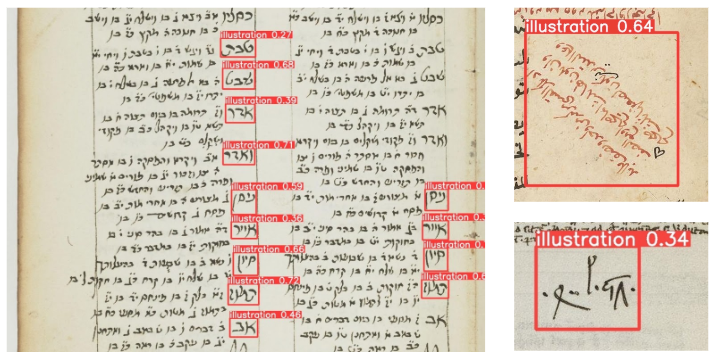
\includegraphics[height=6cm]{figues/marginalia.png}
          \end{center}
          \caption{Détection erronée des marginalia.}
          \label{fig:marginalia} \end{figure}

En outre, le modèle ne parvient pas à détecter les diagrammes occupant
une page entière~: \yolo est en effet conçu pour segmenter une page, ce
qui devient problématique lorsqu'il rencontre des diagrammes l'occupant
entièrement. Le problème vient en outre de la quantité de cas
représentatifs~: les sources contiennent peu de diagrammes en pleine
page. Pour remédier à ce problème, une solution consiste à créer de
fausses illustrations en pleine page en prenant les diagrammes déjà
extraits et en étendant leurs marges, générant ainsi une \textit{groundtruth}
artificielle.

Ces données synthétique peuvent en effet s'avérer cruciales pour
l'entraînement des modèles, afin d'éviter le \textit{sur-apprentissage}, car de
manière générale, prévenir l'\textit{overfitting} implique très souvent
d'augmenter le volume de donnée~; volume qui fait défaut dans le cas des
données historiques. C'est ce que nous détaillons ci-après.
